%<dscrpt>Fichier de déclarations Latex à inclure au début d'un élément de cours.</dscrpt>

\documentclass[a4paper]{article}
\usepackage[hmargin={1.8cm,1.8cm},vmargin={2.4cm,2.4cm},headheight=13.1pt]{geometry}

%includeheadfoot,scale=1.1,centering,hoffset=-0.5cm,
\usepackage[pdftex]{graphicx,color}
\usepackage[french]{babel}
%\selectlanguage{french}
\addto\captionsfrench{
  \def\contentsname{Plan}
}
\usepackage{fancyhdr}
\usepackage{floatflt}
\usepackage{amsmath}
\usepackage{amssymb}
\usepackage{amsthm}
\usepackage{stmaryrd}
%\usepackage{ucs}
\usepackage[utf8]{inputenc}
%\usepackage[latin1]{inputenc}
\usepackage[T1]{fontenc}


\usepackage{titletoc}
%\contentsmargin{2.55em}
\dottedcontents{section}[2.5em]{}{1.8em}{1pc}
\dottedcontents{subsection}[3.5em]{}{1.2em}{1pc}
\dottedcontents{subsubsection}[5em]{}{1em}{1pc}

\usepackage[pdftex,colorlinks={true},urlcolor={blue},pdfauthor={remy Nicolai},bookmarks={true}]{hyperref}
\usepackage{makeidx}

\usepackage{multicol}
\usepackage{multirow}
\usepackage{wrapfig}
\usepackage{array}
\usepackage{subfig}


%\usepackage{tikz}
%\usetikzlibrary{calc, shapes, backgrounds}
%pour la présentation du pseudo-code
% !!!!!!!!!!!!!!      le package n'est pas présent sur le serveur sous fedora 16 !!!!!!!!!!!!!!!!!!!!!!!!
%\usepackage[french,ruled,vlined]{algorithm2e}

%pr{\'e}sentation du compteur de niveau 2 dans les listes
\makeatletter
\renewcommand{\labelenumii}{\theenumii.}
\renewcommand{\thesection}{\Roman{section}.}
\renewcommand{\thesubsection}{\arabic{subsection}.}
\renewcommand{\thesubsubsection}{\arabic{subsubsection}.}
\makeatother


%dimension des pages, en-t{\^e}te et bas de page
%\pdfpagewidth=20cm
%\pdfpageheight=14cm
%   \setlength{\oddsidemargin}{-2cm}
%   \setlength{\voffset}{-1.5cm}
%   \setlength{\textheight}{12cm}
%   \setlength{\textwidth}{25.2cm}
   \columnsep=1cm
   \columnseprule=0.5pt

%En tete et pied de page
\pagestyle{fancy}
\lhead{MPSI-\'Eléments de cours}
\rhead{\today}
%\rhead{25/11/05}
\lfoot{\tiny{Cette création est mise à disposition selon le Contrat\\ Paternité-Pas d'utilisations commerciale-Partage des Conditions Initiales à l'Identique 2.0 France\\ disponible en ligne http://creativecommons.org/licenses/by-nc-sa/2.0/fr/
} }
\rfoot{\tiny{Rémy Nicolai \jobname}}


\newcommand{\baseurl}{http://back.maquisdoc.net/data/cours\_nicolair/}
\newcommand{\urlexo}{http://back.maquisdoc.net/data/exos_nicolair/}
\newcommand{\urlcours}{https://maquisdoc-math.fra1.digitaloceanspaces.com/}

\newcommand{\N}{\mathbb{N}}
\newcommand{\Z}{\mathbb{Z}}
\newcommand{\C}{\mathbb{C}}
\newcommand{\R}{\mathbb{R}}
\newcommand{\D}{\mathbb{D}}
\newcommand{\K}{\mathbf{K}}
\newcommand{\Q}{\mathbb{Q}}
\newcommand{\F}{\mathbf{F}}
\newcommand{\U}{\mathbb{U}}
\newcommand{\p}{\mathbb{P}}


\newcommand{\card}{\mathop{\mathrm{Card}}}
\newcommand{\Id}{\mathop{\mathrm{Id}}}
\newcommand{\Ker}{\mathop{\mathrm{Ker}}}
\newcommand{\Vect}{\mathop{\mathrm{Vect}}}
\newcommand{\cotg}{\mathop{\mathrm{cotan}}}
\newcommand{\sh}{\mathop{\mathrm{sh}}}
\newcommand{\ch}{\mathop{\mathrm{ch}}}
\newcommand{\argsh}{\mathop{\mathrm{argsh}}}
\newcommand{\argch}{\mathop{\mathrm{argch}}}
\newcommand{\tr}{\mathop{\mathrm{tr}}}
\newcommand{\rg}{\mathop{\mathrm{rg}}}
\newcommand{\rang}{\mathop{\mathrm{rg}}}
\newcommand{\Mat}{\mathop{\mathrm{Mat}}}
\newcommand{\MatB}[2]{\mathop{\mathrm{Mat}}_{\mathcal{#1}}\left( #2\right) }
\newcommand{\MatBB}[3]{\mathop{\mathrm{Mat}}_{\mathcal{#1} \mathcal{#2}}\left( #3\right) }
\renewcommand{\Re}{\mathop{\mathrm{Re}}}
\renewcommand{\Im}{\mathop{\mathrm{Im}}}
\renewcommand{\th}{\mathop{\mathrm{th}}}
\newcommand{\repere}{$(O,\overrightarrow{i},\overrightarrow{j},\overrightarrow{k})$}
\newcommand{\cov}{\mathop{\mathrm{Cov}}}

\newcommand{\absolue}[1]{\left| #1 \right|}
\newcommand{\fonc}[5]{#1 : \begin{cases}#2 \rightarrow #3 \\ #4 \mapsto #5 \end{cases}}
\newcommand{\depar}[2]{\dfrac{\partial #1}{\partial #2}}
\newcommand{\norme}[1]{\left\| #1 \right\|}
\newcommand{\se}{\geq}
\newcommand{\ie}{\leq}
\newcommand{\trans}{\mathstrut^t\!}
\newcommand{\val}{\mathop{\mathrm{val}}}
\newcommand{\grad}{\mathop{\overrightarrow{\mathrm{grad}}}}

\newtheorem*{thm}{Théorème}
\newtheorem{thmn}{Théorème}
\newtheorem*{prop}{Proposition}
\newtheorem{propn}{Proposition}
\newtheorem*{pa}{Présentation axiomatique}
\newtheorem*{propdef}{Proposition - Définition}
\newtheorem*{lem}{Lemme}
\newtheorem{lemn}{Lemme}

\theoremstyle{definition}
\newtheorem*{defi}{Définition}
\newtheorem*{nota}{Notation}
\newtheorem*{exple}{Exemple}
\newtheorem*{exples}{Exemples}


\newenvironment{demo}{\renewcommand{\proofname}{Preuve}\begin{proof}}{\end{proof}}
%\renewcommand{\proofname}{Preuve} doit etre après le begin{document} pour fonctionner

\theoremstyle{remark}
\newtheorem*{rem}{Remarque}
\newtheorem*{rems}{Remarques}

\renewcommand{\indexspace}{}
\renewenvironment{theindex}
  {\section*{Index} %\addcontentsline{toc}{section}{\protect\numberline{0.}{Index}}
   \begin{multicols}{2}
    \begin{itemize}}
  {\end{itemize} \end{multicols}}


%pour annuler les commandes beamer
\renewenvironment{frame}{}{}
\newcommand{\frametitle}[1]{}
\newcommand{\framesubtitle}[1]{}

\newcommand{\debutcours}[2]{
  \chead{#1}
  \begin{center}
     \begin{huge}\textbf{#1}\end{huge}
     \begin{Large}\begin{center}Rédaction incomplète. Version #2\end{center}\end{Large}
  \end{center}
  %\section*{Plan et Index}
  %\begin{frame}  commande beamer
  \tableofcontents
  %\end{frame}   commande beamer
  \printindex
}


\makeindex
\begin{document}
\noindent

\debutcours{Géométrie élémentaire du plan}{beta}

\section{Introduction}
\subsection{Points et vecteurs}
Dans cette section $\mathcal P$ désigne un plan. On ne précisera pas davantage ici et on s'appuiera sur les pratiques géométriques des classes précédentes. On devrait dire d'ailleurs plan affine euclidien orienté. Une définition d'un \href{\baseurl C5727.pdf}{espace affine} est donnée dans une autre section.  

La définition d'un plan géométrique fait intervenir un \emph{plan vectoriel sous-jacent} dont les éléments sont des \emph{vecteurs}. Ce plan vectoriel est noté $E$.
\begin{itemize}                                                                                                                                                 \item \`A deux points $M$ et $N$, on peut associer un vecteur noté $\overrightarrow{MN}$. On peut aussi noter simplement $N - M$. La principale propriété est la relation de Chasles.
\item \`A un point $M$ et un vecteur $\overrightarrow u$, on peut associer un point noté $M + \overrightarrow u$.
\item Le plan vectoriel est \emph{euclidien} c'est à dire muni d'un \emph{produit scalaire} ce qui permet de définir l'orthogonalité de deux vecteurs et la norme d'un vecteur. Le plan vectoriel est \emph{orienté} ce qui permet de définir des couples de vecteurs \emph{directs} ou \emph{indirects} ainsi une application \emph{déterminant}.                                                                                                                                                     \end{itemize}
\begin{defi}[base]
 Une base du plan vectoriel sous-jacent est un couple de vecteurs vérifiant certaines propriétés. On dira que $(\overrightarrow u, \overrightarrow v)$ est une base si et seulement si, pour tout vecteur $\overrightarrow w$, il existe un unique couple $(\lambda,\mu)$ de réels tels que :
\begin{displaymath}
 \overrightarrow w = \lambda \overrightarrow u + \mu \overrightarrow v
\end{displaymath}
Les réels $\lambda$ et $\mu$ sont appelés les coordonnées de $\overrightarrow w$ dans la base.
\end{defi}
\begin{defi}
 Une base est dite \emph{orthogonale} lorsque ses vecteurs sont orthogonaux et \emph{orthonormale} ou \emph{orthonormée} lorsque ses vecteurs sont de norme $1$. Un vecteur de norme $1$ est dit \emph{normé} ou \emph{unitaire}. 
\end{defi}
\begin{rem}
 On ne donne pas vraiment de définition ici de ce qu'est une base directe ou indirecte. On se contentera de la figure \ref{fig:C2005_4}.
\end{rem}
\begin{figure}[ht]
 \centering
 \input{C2005_4.pdf_t}
 \caption{Bases directes et indirectes}
 \label{fig:C2005_4}
\end{figure}
\begin{defi}[repère]
 Un repère (cartésien) est un couple formé par un point et une base. Un repère définit des fonctions coordonnées qui permettent de repèrer les points du plan.\newline
Soit $\mathcal R = \left(A,(\overrightarrow u , \overrightarrow v) \right)$ un repère. Il existe alors des fonctions $x$ et $y$ dites \emph{fonctions coordonnées} telles que
\begin{displaymath}
 \forall M\in \mathcal P : \overrightarrow{AM}=x(M)\overrightarrow u + y(M)\overrightarrow v
\end{displaymath}
\end{defi}
\begin{rem}
 Les fonctions coordonnées définies par un repère cartésien constituent un cas particulier de \href{\baseurl C2268.pdf}{système de coordonnées}. Un système de coordonnées est un couple de fonctions dont les valeurs permettent de repérer un point. Ce concept est très important en calcul différentiel.
\end{rem}

\subsection{Fonctions}
Plusieurs types de fonctions peuvent intervenir. Elles jouent des rôles très différents.
\begin{itemize}
 \item du plan dans lui même (transformations géométriques : translations, rotations, homothéties, ...). On peut composer de telles fonctions.
 \item du plan dans $\R$ par exemple les fonctions coordonnées dans un repère ou les fonctions constantes à valeurs réelles. On peut additionner et multiplier (entre elles ou par un scalaire) de telles fonctions. En revanche on ne peut pas les composer.
 \item d'un intervalle de $\R$ dans un plan. Par exemple, si on se donne un point $A$ et un vecteur $\overrightarrow u$, on peut considérer une fonction $t\rightarrow A + t\overrightarrow u$. Ou encore, si on se donne un nombre complexe $z$ non réel, on peut considérer la fonction qui à tout réel $t$ associe le point d'affixe $\frac{1}{t-z}$.   
\end{itemize}

\subsection{Parties d'un plan}
Ensembles de points . Exemple : les droites, les cercles sont des ensembles de points.

\'Equation cartésienne ou représentation paramétrique d'une partie du plan. Lignes de niveau d'une fonction.

\section{Modes de repérage}
\subsection{Repère polaire}
\begin{defi}
 Un repère orthonormé direct $\mathcal{R}=\left(O,(\overrightarrow i , \overrightarrow j) \right)$ étant fixé, on note
\begin{displaymath}
 \overrightarrow{e_\theta} = \cos\theta \overrightarrow i +\sin\theta \overrightarrow j
\end{displaymath}
\end{defi}
\begin{rems}
 \begin{enumerate}
  \item  Cette notation est choisie pour être la plus proche possible de l'exponentielle complexe. Pour la base orthonormale fixée, l'affixe du vecteur $\overrightarrow{e_\theta}$ est le complexe $e^{i\theta}$. 
\item Le couple $\left( \overrightarrow{e_\theta}, \overrightarrow{e_{\theta + \frac{\pi}{2}}}\right)$ est une base orthonormée directe.  
 \end{enumerate}
\end{rems}
\begin{prop}
 Pour tous $\theta$ et $\varphi$ réels :
\begin{displaymath}
 \cos \varphi \,\overrightarrow{e_\theta} + \sin \varphi \,\overrightarrow{e_{\theta + \frac{\pi}{2}}}
= \overrightarrow{e_{\theta + \varphi}}  
\end{displaymath}
\end{prop}
\begin{demo}
 On passe en affixes :
\begin{displaymath}
 \cos \theta e^{i\theta} + \sin \theta i e^{i\theta} = e^{i\varphi}e^{i\theta}= e^{i(\theta + \varphi)}
\end{displaymath}

\end{demo}

\subsection{Changement de repère}
\index{qc changement de repère}
\begin{prop}
 Soit $\mathcal{R}=\left(O,(\overrightarrow i , \overrightarrow j) \right)$ et $\mathcal{R}=\left(O_1,(\overrightarrow i_1 , \overrightarrow j_1)\right) $ deux repères. Les fonctions coordonnées dans ces repères sont respectivement notés $(x,y)$ et $(x_1,y_1)$. Il existe alors des réels $a$, $b$, $c$, $a'$, $b'$, $c'$ tels que :
\begin{align*}
\begin{vmatrix}
 a & b \\
 a'& b'
\end{vmatrix}
\neq 0
& &
 \left\lbrace 
\begin{aligned}
 x &= a x_1 + a'y_1 + c \\
 y &= b x_1 + b' y_1 + c'  
\end{aligned}
\right. 
\end{align*}
\end{prop}
\begin{demo}
 Comme $(\overrightarrow i , \overrightarrow j)$ est une base, il existe des réels $a$, $b$, $a'$, $b$ permettant d'exprimer les vecteurs $\overrightarrow i_1$ et $\overrightarrow j_1$. On peut ensuite les combiner linéairement avec les coordonnées d'un point $M$ quelconque :
\begin{multline*} 
\left. 
 \begin{aligned}
  \overrightarrow i_1 &= a\overrightarrow i + b \overrightarrow j &\times x_1(M)\\
  \overrightarrow j_1 &= a'\overrightarrow i + b' \overrightarrow j &\times y_1(M)\\
  \overrightarrow{OO_1}&=x(O_1)\overrightarrow i +y(O_1)\overrightarrow j &
 \end{aligned}
\right\rbrace 
\Rightarrow
\overrightarrow{O_1M}
= \left(ax_1(M)+a'y_1(M) \right)\overrightarrow i +
  \left(bx_1(M)+b'y_1(M) \right)\overrightarrow j  
\\
\Rightarrow
\overrightarrow{OM}
= \underset{= x(M)}{\underbrace{\left(ax_1(M)+a'y_1(M) +x(O_1)\right)}}\overrightarrow i +
  \underset{ = y(M)}{\underbrace{\left(bx_1(M)+b'y_1(M) +y(O_1)\right)}}\overrightarrow j  
\end{multline*}
On termine en passant d'une famille d'égalités numériques (entre des réels) à des égalités fonctionnelles (entre des fonctions).
\begin{displaymath}
\left(
\forall M\in \mathcal{P} :
\left\lbrace 
\begin{aligned}
 x(M) &= ax_1(M)+a'y_1(M) +x(O_1)\\
 y(M) &= bx_1(M)+b'y_1(M) +y(O_1)
\end{aligned} \right. 
\right) 
\Leftrightarrow
\left\lbrace 
\begin{aligned}
 x &= ax_1 + a'y_1 +x(O_1)\\
 y &= bx_1+b'y_1 +y(O_1)
\end{aligned} \right. 
\end{displaymath}
Le déterminant est non nul car chaque système linéaire (associé à un point $M$) admet un unique couple de solutions.
\end{demo}
\begin{rem}
\begin{itemize}
 \item Dans la démonstration précédente, on s'est donné au départ les expressions dans $\mathcal{R}$ des objets de $\mathcal{R}_1$. Le calcul a conduit à l'expression des coordonnées $x$ et $y$ dans $\mathcal{R}$ en fonction des coordonnées dans $\mathcal{R}_1$.
 \item Quand on veut \emph{changer de repère} et passer de $\mathcal{R}$ à $\mathcal{R}_1$. En général, on connait les objets de $\mathcal{R}_1$ en fonction de ceux de $\mathcal{R}$ et on veut $x_1$ et $y_1$ en fonction de $x$ et $y$. \emph{Une inversion est nécessaire}. Elle peut se faire au début ou à la fin. 
\end{itemize}
\end{rem}
\subparagraph{Pratique}
\begin{enumerate}
 \item Exemple de changement de repère. Les fonctions coordonnées dans le repère $\mathcal{R}=(O,\overrightarrow i , \overrightarrow j)$ sont désignées par $x$ et $y$. On définit un nouveau repère $\mathcal{R}_1=(A,\overrightarrow u , \overrightarrow v)$ par les relations
\begin{displaymath}
 x(A)=0, y(A)=1\hspace{1cm} \overrightarrow u = \overrightarrow i +\overrightarrow j , \overrightarrow v = \overrightarrow i
\end{displaymath}
On désigne par $(X,Y)$ les fonctions coordonnées dans $\mathcal{R}_1$. Exprimer $(x,y)$ en fonction de $X$ et $Y$ puis $X$ et $Y$ en fonction de $x$ et $y$.
 \item Inversement, il peut être commode dans un calcul de poser
\begin{align*}
 x_1=u+ax+by & & y_1=v+cy+dy
\end{align*}
avec $a$, $b$, $c$, $d$, $u$, $v$ six nombres réels particuliers tels que 
\begin{displaymath}
 \begin{vmatrix}
  a & b \\
c & d
 \end{vmatrix}
\neq 0
\end{displaymath}
Le couple $(x_1,y_1)$ est-il un système de coordonnées cartésiennes et dans quel repère ?\newline
La réponse est oui, c'est bien un système de coordonnées. Pour déterminer pratiquement le repère $\mathcal R_1=(O_1,\overrightarrow{i_1},\overrightarrow{j_1})$ auquel il est associé, on considère les points $I_1$ et $J_1$ tels que
\begin{align*}
 \overrightarrow{i_1}=\overrightarrow{O_1I_1} & & \overrightarrow{j_1}=\overrightarrow{O_1J_1}
\end{align*}
En résolvant des systèmes, on calcule les coordonnées dans $\mathcal R$ des points $O_1$, $I_1$, $J_1$ en utilisant:
\begin{align*}
 \left\lbrace 
\begin{aligned}
 x_1(O_1)=& 0\\
 y_1(O_1)=& 0
\end{aligned}
\right. 
& & 
 \left\lbrace 
\begin{aligned}
 x_1(I_1)=& 1\\
 y_1(I_1)=& 0
\end{aligned}
\right. 
& & 
 \left\lbrace 
\begin{aligned}
 x_1(J_1)=& 0\\
 y_1(J_1)=& 1
\end{aligned}
\right. 
\end{align*}
Exemple On définit des fonctions $X$ et $Y$ par
\begin{displaymath}
 \left\lbrace 
\begin{aligned}
 X &= 1+x+y \\ Y = 2+2x-y
\end{aligned}
\right. 
\end{displaymath}
Préciser l'origine et la base d'un repère pour lequel $X$ et $Y$ sont les fonctions coordonnées.
\item Un cas particulier important est celui des repère orthonormés directs de même origine. Si $\overrightarrow{i_1}=\overrightarrow{e_\theta}$, alors :
\begin{align*}
 \left\lbrace 
\begin{aligned}
 \overrightarrow{i_1} =& \cos \theta  \overrightarrow{i} + \sin \theta  \overrightarrow{j} \\ 
\overrightarrow{j_1} =& -\sin \theta  \overrightarrow{i} + \cos \theta  \overrightarrow{j}
\end{aligned}
\right.
& &
 \left\lbrace 
\begin{aligned}
 x =& x_1\cos \theta   - y_1\sin \theta \\ 
 y =& x_1\sin \theta   + y_1\cos \theta 
\end{aligned}
\right.
\end{align*}
Ces formules s'inversent simplement en changeant $\theta$ en $-\theta$.
\begin{align*}
 \left\lbrace 
\begin{aligned}
 \overrightarrow{i} =& \cos \theta  \overrightarrow{i_1} - \sin \theta  \overrightarrow{j_1} \\ 
\overrightarrow{j} =& \sin \theta  \overrightarrow{i_1} + \cos \theta  \overrightarrow{j_1}
\end{aligned}
\right.
& &
 \left\lbrace 
\begin{aligned}
 x_1 =& x\cos \theta   + y\sin \theta \\ 
 y_1 =& -x\sin \theta   + y\cos \theta 
\end{aligned}
\right.
\end{align*}
\end{enumerate}

\subsection{Coordonnées polaires}
Les fonctions coordonnées polaires souffrent d'un défaut inévitable lié à la malédiction du logarithme. On ne peut pas les définir de manière satisfaisante dans le plan tout entier. Un repère orthonormal direct étant fixé, on ne definit les fonctions $\rho$ et $\theta$ que dans le plan \emph{fendu} c'est à dire privé de la demi droite constituée des points $M$ tels que $x(M)\leq 0$ et $y(M)=0$. Dans ces conditions $\rho$ est à valeurs dans $]0,+\infty$ et $\theta$ dans $]-\pi,\pi[$.

En revanche, on peut définir un unique point $M$ à partir d'un nombre $\rho >0$ et d'un nombre $\theta$ quelconque par la relation
\begin{displaymath}
 \overrightarrow{OM} = \rho \overrightarrow{e}_\theta
\end{displaymath}
Ces nombres sont souvent désignés comme les coordonnées polaires de $M$ mais cela prète à confusion. Quoiqu'il en soit utilisons les pour caractériser que $M$ est sur une droite ou un cercle. 
\begin{center}
\renewcommand{\arraystretch}{1.5}
\begin{tabular}{|l|l|}\hline
droite passant par $O$ & $\theta \equiv \alpha \mod \pi$ pour $\alpha$ fixé\\ \hline
droite ne passant pas par $O$ & $\rho(A\cos \theta + B\sin \theta) = 1$ pour $A$ et $B$ réels fixés\\ \hline
cercle passant par $O$ & $\rho = A\cos \theta + B\sin \theta$ pour $A$ et $B$ réels fixés\\ \hline
cercle centré en $O$ & $\rho = R$ pour $R>0$ fixé \\ \hline
\end{tabular}
\end{center}

\section{Produit scalaire et déterminant}
\subsection{Produit scalaire}
On admet la proposition suivante qui sert aussi de définition.
\begin{prop}
 Il existe une application
\begin{displaymath}
 \begin{aligned}
  E\times E \rightarrow& \R \\
  (\overrightarrow{u},\overrightarrow{v}) \rightarrow& (\overrightarrow{u}/\overrightarrow{v})
 \end{aligned}
\end{displaymath}
telle que :
\begin{align*}
 \forall (\overrightarrow{u},\overrightarrow{v})\in E^2 : (\overrightarrow{u}/\overrightarrow{v})=(\overrightarrow{v}/\overrightarrow{u}) & &\text{(symétrique)}\\
\left. 
\begin{aligned}
 \forall (\overrightarrow{u},\overrightarrow{v},\overrightarrow{w})\in E^3 &:&
(\overrightarrow{u}+\overrightarrow{v}/\overrightarrow{w})=(\overrightarrow{u}/\overrightarrow{w})+(\overrightarrow{v}/\overrightarrow{w})\\
\forall \lambda \in \R &:&  (\lambda\overrightarrow{u}/\overrightarrow{v})=\lambda(\overrightarrow{u}/\overrightarrow{v})
\end{aligned}
\right\rbrace  & & \text{(linéarité première place)} \\
\left. 
\begin{aligned}
 \forall (\overrightarrow{u},\overrightarrow{v},\overrightarrow{w})\in E^3 &:&
(\overrightarrow{u}/\overrightarrow{v}+\overrightarrow{w})=(\overrightarrow{u}/\overrightarrow{v})+(\overrightarrow{u}/\overrightarrow{w})\\
\forall (\overrightarrow{u},\overrightarrow{v})\in E^2, \forall \lambda \in \R &:&  (\overrightarrow{u}/\lambda\overrightarrow{v})=\lambda(\overrightarrow{u}/\overrightarrow{v})
\end{aligned}
\right\rbrace  & & \text{(linéarité deuxième place)} \\
\forall \overrightarrow{u}\in E :
\left. 
 \begin{aligned}
  (\overrightarrow{u}/\overrightarrow{u})\geq& 0 \\
(\overrightarrow{u}/\overrightarrow{u})=0\Leftrightarrow& \overrightarrow{u}=\overrightarrow{0}
 \end{aligned}
 \right\rbrace & & \text{(définie positive)}
\end{align*}
\end{prop}
On définit alors la norme d'un vecteur :
\begin{displaymath}
 \Vert \overrightarrow{u}\Vert = \sqrt{(\overrightarrow{u}/\overrightarrow{u})}
\end{displaymath}
Deux vecteurs sont orthogonaux si et seulement si leur produit scalaire est nul. Une base est dite \emph{orthogonale} si et seulement si elle est formée de vecteurs orthogonaux. Une base est dite \emph{orthonormée} si et seulement si elle est formée de vecteurs orthogonaux et de norme $1$.
\begin{prop}
 Soit $(\overrightarrow i, \overrightarrow j)$ une base orthonormée, le produit scalaire de deux vecteurs s'exprime dans une telle base :
\begin{displaymath}
 \left. 
\begin{aligned}
 \overrightarrow u &= x\overrightarrow i + y\overrightarrow j \\
 \overrightarrow u' &= x'\overrightarrow i + y'\overrightarrow j 
\end{aligned}
\right\rbrace \Rightarrow
(\overrightarrow u / \overrightarrow v) = xx'+yy'
\end{displaymath}
\end{prop}
\begin{demo}
 C'est une conséquence immédiate de la symétrie et de la bilinéarité.
\end{demo}
Une orientation du plan étant fixée, on admet la propriété suivante
\begin{prop}
 Pour tout vecteur normé $\overrightarrow{u}$, il existe un unique vecteur normé $\overrightarrow{v}$ tel que $(\overrightarrow{u},\overrightarrow{v})$ soit une base orthonormée directe.
\end{prop}
\begin{defi}[Angle orienté de deux vecteurs]
 Soit $\overrightarrow u$ et $\overrightarrow v$ deux vecteurs non nuls. On pose
\begin{displaymath}
 \overrightarrow{u_1}=\dfrac{1}{\Vert\overrightarrow{u}\Vert}\overrightarrow{u}
\end{displaymath}
et $\overrightarrow{v_1}$ est l'unique vecteur tel que $(\overrightarrow{u_1},\overrightarrow{v_1})$ soit une base orthonormé. Il existe alors des réels $\alpha$ (congrus modulo $2\pi$) tels que
\begin{displaymath}
 \overrightarrow{u} = \cos\alpha \overrightarrow{u_1} + \sin\alpha \overrightarrow{v_1}
\end{displaymath}
Cette classe de nombres modulo $2\pi$ est l'angle orienté entre les deux vecteurs, on peut le noter $\widehat{(\overrightarrow{u},\overrightarrow{v})}$, les nombres $\alpha$ sont appelés des mesures de l'angle.
\end{defi}
On vérifie facilement à l'aide de la fonction exponentielle complexes les propriétés suivantes. Si $\alpha$ est une mesure de $\widehat{(\overrightarrow{u},\overrightarrow{v})}$ alors $-\alpha$ est une mesure de $\widehat{(\overrightarrow{v},\overrightarrow{u})}$. De même, si $\alpha$ est une mesure de $\widehat{(\overrightarrow{u},\overrightarrow{v})}$ et $\beta$ est une mesure de $\widehat{(\overrightarrow{v},\overrightarrow{w})}$ alors $\alpha + \beta$ est une mesure de $\widehat{(\overrightarrow{u},\overrightarrow{w})}$.
\begin{prop}
 Si $\overrightarrow u$ et $\overrightarrow v$ sont deux vecteurs non nuls et si $\alpha$ est une mesure de l'angle orienté $\widehat{(\overrightarrow{u},\overrightarrow{v})}$ alors
\begin{displaymath}
 (\overrightarrow{u}/\overrightarrow{v}) = \Vert\overrightarrow{u}\Vert \Vert\overrightarrow{v}\Vert \cos \alpha
\end{displaymath}
\end{prop}
Inégalité de Cauchy-Schwarz. \'Ecart angulaire. Exemples deux figures avec $\frac{2\pi}{3}$ et $-\frac{2\pi}{3}$.

\subsection{Déterminant}
On admet la proposition suivante qui sert aussi de définition.
\begin{prop}
Il existe une application notée $\det$ de $E\times E$ dans $\R$ qui vérifie les propriétés suivantes.
\begin{align*}
 \forall (\overrightarrow{u},\overrightarrow{v})\in E^2 : \det(\overrightarrow{u},\overrightarrow{v})=
-\det(\overrightarrow{v},\overrightarrow{u}) & &\text{(antisymétrique)}\\
\left. 
\begin{aligned}
 \forall (\overrightarrow{u},\overrightarrow{v},\overrightarrow{w})\in E^3 &:&
\det(\overrightarrow{u}+\overrightarrow{v},\overrightarrow{w})=\det(\overrightarrow{u},\overrightarrow{w})+\det(\overrightarrow{v},\overrightarrow{w})\\
\forall \lambda \in \R &:&  \det(\lambda\overrightarrow{u},\overrightarrow{v})=\lambda\det(\overrightarrow{u},\overrightarrow{v})
\end{aligned}
\right\rbrace  & & \text{(linéarité première place)} \\
\left. 
\begin{aligned}
 \forall (\overrightarrow{u},\overrightarrow{v},\overrightarrow{w})\in E^3 &:&
\det(\overrightarrow{u},\overrightarrow{v}+\overrightarrow{w})=\det(\overrightarrow{u},\overrightarrow{v})+\det(\overrightarrow{u},\overrightarrow{w})\\
\forall (\overrightarrow{u},\overrightarrow{v})\in E^2, \forall \lambda \in \R &:&  \det(\overrightarrow{u},\lambda\overrightarrow{v})=\lambda\det(\overrightarrow{u},\overrightarrow{v})
\end{aligned}
\right\rbrace  & & \text{(linéarité deuxième place)}
\end{align*}
De plus, pour toute base orthonormée $(\overrightarrow u, \overrightarrow v)$ directe :
\begin{displaymath}
 \det(\overrightarrow u, \overrightarrow v) = 1
\end{displaymath}
\end{prop}
\begin{prop}
 Soit $(\overrightarrow i, \overrightarrow j)$ une base orthonormée directe quelconque, le produit scalaire de deux vecteurs s'exprime dans une telle base :
\begin{displaymath}
 \left. 
\begin{aligned}
 \overrightarrow u &= x\overrightarrow i + y\overrightarrow j \\
 \overrightarrow u' &= x'\overrightarrow i + y'\overrightarrow j 
\end{aligned}
\right\rbrace \Rightarrow
\det(\overrightarrow u , \overrightarrow v) = 
\begin{vmatrix}
 x & x' \\
 y & y'
\end{vmatrix}
\end{displaymath}
\end{prop}
\begin{demo}
 C'est une conséquence de la bilinéarité et de l'antisymétrie.
\end{demo}
\begin{prop}
 Si $\overrightarrow u$ et $\overrightarrow v$ sont deux vecteurs non nuls et si $\alpha$ est une mesure de l'angle orienté $\widehat{(\overrightarrow{u},\overrightarrow{v})}$ alors
\begin{displaymath}
 \det(\overrightarrow{u},\overrightarrow{v}) = \Vert\overrightarrow{u}\Vert \Vert\overrightarrow{v}\Vert \sin \alpha
\end{displaymath}
\end{prop}
\begin{demo}
 On pose $\overrightarrow{u_1} = \frac{1}{\Vert \overrightarrow u \Vert}\overrightarrow u$ et on considère la base orthonormée directe $(\overrightarrow {u_1}, \overrightarrow{w})$. \'Ecrivons les coordonnées dans cette base :
\begin{displaymath}
\left. 
\begin{aligned}
 \overrightarrow u &= \Vert \overrightarrow u \Vert \overrightarrow{u_1} \\
 \overrightarrow v &= \cos \alpha \overrightarrow{u_1} + \sin \alpha \overrightarrow{w}
\end{aligned}
\right\rbrace \Rightarrow
\det (\overrightarrow{u},\overrightarrow{v}) =
\begin{vmatrix}
 \Vert \overrightarrow u \Vert & \cos \alpha \\
 0 & \sin\alpha
\end{vmatrix}
= \Vert \overrightarrow u \Vert \sin \alpha
\end{displaymath}

\end{demo}

\subsubsection*{Intoduction à la notion d'aire}
$\mathcal A (\Omega)$ est un nombre réel positif défini pour certaines parties $\Omega$ du plan. On ne cherchera pas à préciser lesquelles ici. Cette fonction doit vérifier des propriétés qui la déterminent complètement et permettent de faire des calculs.
\begin{figure}[ht]
 \centering
\input{C2005_2.pdf_t}
\caption{Aire d'un parallélogramme}
\label{fig:C2005_2}
\end{figure}

\begin{description}
 \item Aire d'un rectangle
\item Additivité
\item Invariance par isométrie.
\end{description}

\section{Droites et cercles}
\subsection{Droites}
\subsubsection{Définition paramétrique}
Angle orienté de droites
\subsubsection{\'Equation cartésienne}
vecteur directeur : déterminant 

vecteur normal : produit scalaire (équation "normale")

Inversement: toute équation de la forme $ax+by+c$ avec $(a,b)\neq (0,0)$ est celle d'une droite.
\subsubsection{Intersection de deux droites}
Si les droites sont données pa deux équations cartésiennes, il s'agit de résoudre un système linéaire de deux équations.

Si une droite est donnée par une équation cartésienne et l'autre est définie paramétriquement, on substitue l'expression paramétrique dans l'équation et on en déduit la valeur du paramètre pour le point d'intersection.
\begin{prop}[Projection orthogonale et réflexion]
 
\end{prop}
\index{distance d'un point à une droite dans un plan}
\begin{prop}[Distance d'un point à une droite]
 
\end{prop}

\begin{prop}[bissectrices]
 
\end{prop}


\subsection{Cercles}
\subsubsection{\'Equation cartésienne}
cas où le cercle passe par l'origine. \'Equation polaire du cercle privé de l'origine.
\subsubsection{Intersection droite-cercle}
On définit la droite paramétriquement et le cercle par une équation. Si on substitue l'expression paramétrique dans l'équation, on obtient une équation du second degré à coefficient réel.
\begin{itemize}
 \item si le discriminant est strictement positif : deux points d'intersection
 \item si le discriminant est nul: un seul point d'intersection, la droite est tangente
 \item si le discriminant est négatif : intersction vide
\end{itemize}
\index{règle du dédoublement pour un cercle}
\begin{prop}[règle du dédoublement pour un cercle]
 Un plan $\mathcal{P}$ est muni d'un repère orthonormé direct $\mathcal{R}$ dont le fonctions coordonnées sont notées $x$ et $y$. Soit $\mathcal C$ un cercle de centre un point $A$ et de rayon $r>0$, soit $M_0$ un point de $\mathcal C$. L'équation de la tangente en $M_0$ au cercle est :
\begin{displaymath}
 \left( x-x(A)\right) \left( x(M_0)-x(A)\right) + \left( y-y(A)\right) \left( y(M_0)-y(A)\right) - r^2 = 0 
\end{displaymath}
\end{prop}
\begin{demo}
 \begin{enumerate}
  \item Si on prend la valeur en $M_0$, on obtient $0$ car c'est l'équation même du cercle et ce cercle contient $M_0$. On en déduit que $M_0$ est dans la ligne de niveau $0$ de la  fonction proposée. 
  \item L'équation proposée est de la forme $ax+by+c=0$ c'est bien celle d'une droite. Le vecteur de coordonnées
\begin{displaymath}
 \left( x(M_0)-x(A), y(M_0)-y(A)\right) 
\end{displaymath}
 est normal à cette droite. Or il s'agit des coordonnées de $\overrightarrow{AM_0}$. On en déduit qu'il s'agit de la tangente en $M_0$ au cercle.
 \end{enumerate}

\end{demo}


\subsubsection{Définitions paramétriques}
Paramétrisation trigonométrique.\newline
Un repère orthonormé étant fixé, un point $M$ est sur un cercle de centre $A$ et de rayon $
r$ si et seulement si il existe un réel $\theta$ tel que 
\begin{displaymath}
 M = A +e\overrightarrow{e_\theta}
\end{displaymath}
Paramétrisation rationnelle.\newline
On obtient une paramétrisation rationnelle d'un cercle privé d'un point $A$ en considérant la famille des droites passant par $A$. Par exemple on peut prendre des droites $(AP_\lambda)$ où $P_\lambda$ décrit une droite qui n'est pas la tangente en $A$. L'intersection du cercle avec $(AP_\lambda)$ est régie par une équation du second degré dont on connait une racine, celle qui correspond au point d'intersection $A$. L'autre point que l'on peut noter $M_\lambda$ dépend rationnellement de $\lambda$. Par exemple dans la figure \ref{fig:C2005_3}, l'origine est en $A$ et le centre a pour coordonnées $(1,0)$.
\begin{figure}[ht]
 \centering
\input{C2005_3.pdf_t}
\caption{Paramétrisation rationnelle d'un cercle}
\label{fig:C2005_3}
\end{figure}
Les coordonnées de $P_\lambda$ sont $(2,\lambda)$. Les coordonnées de $M_\lambda$ sont de la forme $(2k,k\lambda)$. On  injecte ces coordonnées dans l'équation du cercle ce qui conduit à une équation en $k$ :
\begin{displaymath}
 (2k-1)^2+(k\lambda)^2=1\Rightarrow k=\dfrac{4}{4+\lambda^2}
\end{displaymath}
Un point $M$ autre que $A$ est donc sur le cercle si et seulement si il existe un réel $\lambda$ tel que les coordonnées de $M$ soient
\begin{displaymath}
 (\dfrac{8}{4+\lambda^2},\dfrac{8\lambda}{4+\lambda^2})
\end{displaymath}
De plus, le paramètre trigonométrique $\theta$ et le paramètre rationnel $\lambda$ sont reliés ici par $\lambda =2\tan\frac{\theta}{2}$.
\section{Lignes de niveau}
\subsection{Fonction attachée à un produit scalaire.}
$M\rightarrow (\overrightarrow{MA},\overrightarrow{MB})$
\subsection{Fonction attachée à un quotient de deux distances.}
\begin{displaymath}
 M \rightarrow \frac{AM}{BM}
\end{displaymath}

\subsection{Fonction attachée à un angle de droites.}
\begin{figure}[ht]
 \centering
 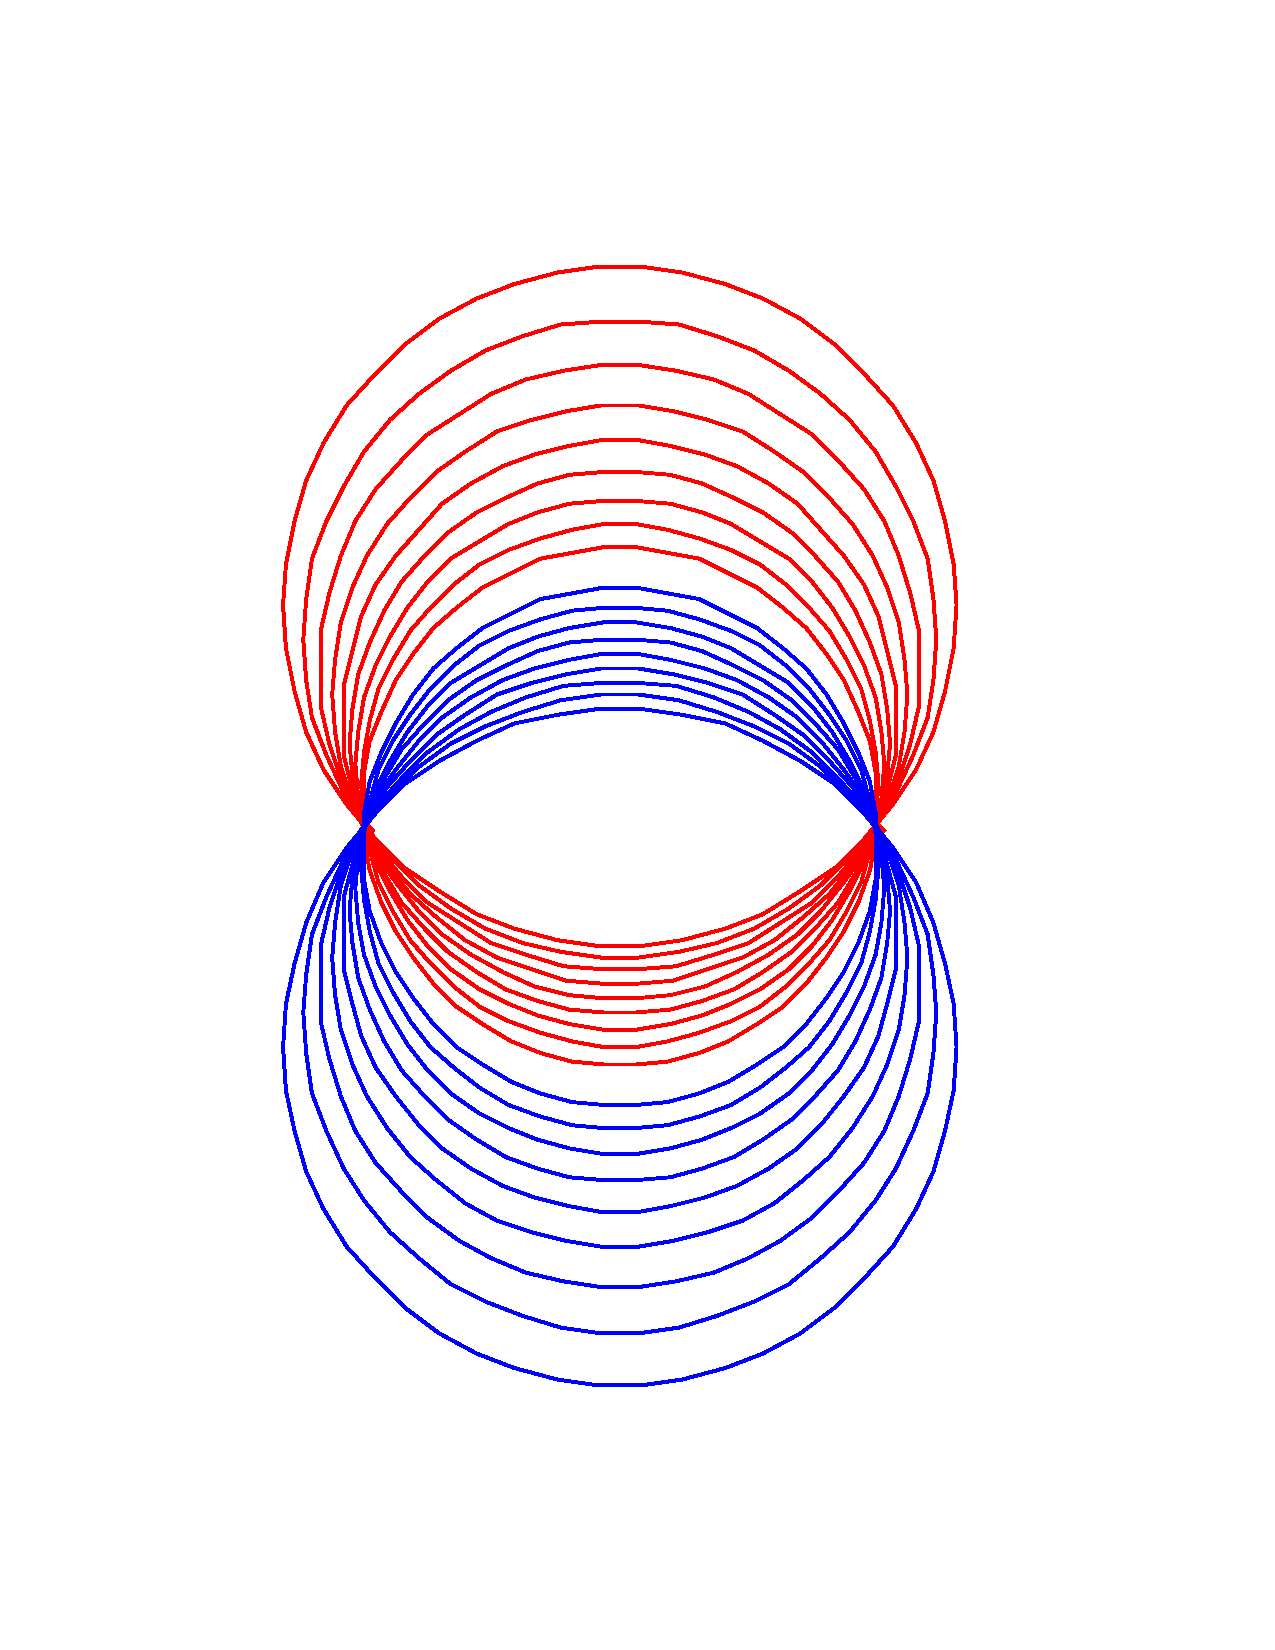
\includegraphics[width=8cm]{C2005_1.pdf}
 \caption{Lignes de niveau pour angle de droites}
\label{fig:C2005_1}
\end{figure}
Ligne de niveau de $ M \rightarrow ((AM),(BM))$ où $((AM),(BM))$ désigne l'angle des deux droites.\newline
En fait :
\begin{displaymath}
 ((AM),(BM)) = \alpha \Leftrightarrow \tan ((AM),(BM))= \tan \alpha
\Leftrightarrow
\dfrac{\det(\overrightarrow{AM},\overrightarrow{BM})}{(\overrightarrow{AM}/\overrightarrow{BM})}
=\tan \alpha
\end{displaymath}
On fait les calculs en utilisant un repère dont l'origine est le milieu de $[A,B]$ et dont le premier vecteur est dirigé de $A$, vers $B$. Les coordonnées de $A$ sont de la forme $(-a,0)$, celles de $B$ de la forme $(a,0)$. Après calculs, la relation s'écrit
\begin{displaymath}
 2ay = \tan\alpha((x^2-a^2)+y^2)
\end{displaymath}
On en déduit que les lignes de niveau sont des cercles dont le centre est sur la médiatrice de $[A,B]$ voir figure \ref{fig:C2005_1}.
\section{Complément: utilisation d'un déterminant}
Ces conditions utilisent les propriétés des déterminants $3\times3$ (voir \href{\baseurl C4199.pdf}{Glossaire de début d'année}).
\subsection{Condition d'alignement}\index{condition d'alignement}
\begin{prop}
 Soient $x$ et $y$ les fonctions coordonnées dans un repère quelconque. Trois points $A$, $B$, $C$ sont alignés si et seulement si
\begin{displaymath}
 \begin{vmatrix}
  x(A) & &y(A) & 1 \\
x(B) & & y(B) & 1 \\
x(C) & & y(C) & 1 
 \end{vmatrix}
=0
\end{displaymath}
\end{prop}
\begin{demo}
Considérons le système d'équations d'inconnues $(u,v,w)$
\begin{align*}
 \left\lbrace 
\begin{aligned}
 x(A)u+ y(A)v + 1c =& 0\\ 
x(B)u+ y(B)v + 1c =& 0\\
x(C)u+ y(C)v + 1c =& 0
\end{aligned}
\right. & & (\mathcal S)
\end{align*}
La nullité du déterminant traduit l'existence d'un triplet $(a,b,c)\neq(0,0,0)$ solution du système $\mathcal S$.\newline
Comme $(a,b,c)\neq(0,0,0)$, si on avait $(a,b)=(0,0)$, on aurait aussi $c\neq0$. Ce qui est incompatible avec le fait que $(a,b,c)$ soit solution de $\mathcal S$. L'équation
\begin{displaymath}
 ax+by+c = 0
\end{displaymath}
 est donc bien celle d'une droite qui contient les points $A$, $B$, $C$. Ils sont donc alignés.

Réciproquement, si les trois points sont alignés, il existe une droite (d'équation $ax+by+c = 0$) qui les contient tous les trois. Alors $(a,b,c)$ est une solution non identiquement nulle  d'un système $\mathcal S$. Le déterminant de ce système est donc nul.
\end{demo}
\subsection{Condition de parallélisme ou de concours}
\begin{prop}
 Soient $x$ et $y$ les fonctions coordonnées dans un repère quelconque. On considère trois droites dont les équations sont :
\begin{align*}
 ax+by+c=&0\\ 
 a'x+b'y+c'=&0 \\
 a''x+b''y+c''=&0
\end{align*}
Ces trois droites sont parallèles ou concourantes si et seulement si
\begin{displaymath}
 \begin{vmatrix}
  a & b & c  \\
  a' & b' & c' \\
  a'' & b'' & c''
 \end{vmatrix}
= 0
\end{displaymath}
\end{prop}
\begin{demo}
 Notons $D$ le déterminant figurant dans la propriété, formons un système de trois équations aux inconnues $(u,v,w)$
\begin{align*}
 (S) \hspace{1cm} \left\lbrace 
\begin{aligned}
 au+bv+cw =&0\\
a'u+b'v+c'w =&0\\
a''u+b''v+c''w =&0
\end{aligned}
\right. 
\end{align*}
On remarque que ce système admet la solution triviale $(0,0,0)$. D'après le résultat fondamental sur les systèmes linéaires de trois équations, la condition $D=0$ est équivalente à l'existence d'une solution $(u,v,w)\neq(0,0,0)$.\\
La preuve est constituée de trois parties
\begin{itemize}
 \item Si les trois droites sont concourantes alors $D=0$.
\item Si les trois droites sont parallèles alors $D=0$.
\item Si $D=0$ alors deux cas apparaissent : dans un les trois droites sont concourantes, dans l'autre elles sont parallèles.
\end{itemize}
Supposons que les trois droites se coupent en un point $A$. \'Ecrire que $A$ appartient à chaque droite conduit à trois relations qui signifient que $(x(A),y(A),1)$ est solution de $(S)$. \`A cause du $1$, cette solution n'est pas $(0,0,0)$ donc $D=0$.\newline
Supposons que les trois droites sont parallèles. Leurs vecteurs directeurs sont donc colinéaires, par exemple proportionnels au premier. On en déduit qu'il existe des réels $\lambda$ et $\mu$ tels que :
\begin{align*}
 a'=\lambda a & & b'=\lambda b & & a''=\mu a & & b'' =\mu b
\end{align*}
On peut alors calculer le déterminant en exploitant la multilinéarité 
\begin{displaymath}
 D =
\begin{vmatrix}
 a & b & c \\
\lambda a & \lambda b & c' \\
\mu a & \mu b & c'' 
\end{vmatrix}
=\begin{vmatrix}
 a & b & c \\
0 & 0 & c'-\lambda c \\
\mu a & \mu b & c'' 
\end{vmatrix}
=\begin{vmatrix}
 a & b & c \\
0 & 0 & c'-\lambda c \\
0 & 0 & c''-\mu c 
\end{vmatrix}=0
\end{displaymath}
car la matrice est triangulaire avec un $0$ sur la diagonale.\\
Supposons maintenant que $D=0$. Il existe donc une solution $(u,v,w)\neq (0,0,0)$.
\begin{itemize}
 \item Si $w\neq 0$. On peut diviser par $w$ et comme les seconds membres sont nuls, $(\frac{u}{w},\frac{v}{w},1)$ est une solution de $(S)$. Le point de coordonnées $(\frac{u}{w},\frac{v}{w})$ appartient alors aux trois droites qui sont concourantes.
\item Si $w= 0$, alors $(u,v)\neq (0,0)$. Considérons un vecteur $\overrightarrow n$ de coordonnées $(u,v)$ (il n'est donc pas nul). Le système s'écrit
\begin{displaymath}
 \left\lbrace 
\begin{aligned}
 au+bv =&0\\
a'u+b'v =&0\\
a''u+b''v =&0
\end{aligned}
\right. 
\end{displaymath}
Ces relations traduisent que les trois vecteurs directeurs des droites (dont les coordonnées sont respectivement $(-b,a)$, $(-b',a')$, $(-b'',a'')$ ) sont colinéaires à $\overrightarrow n$. Cela entraine que les trois droites sont parallèles.
\end{itemize}
\end{demo}
\end{document}
